% Options for packages loaded elsewhere
\PassOptionsToPackage{unicode}{hyperref}
\PassOptionsToPackage{hyphens}{url}
\PassOptionsToPackage{dvipsnames,svgnames,x11names}{xcolor}
%
\documentclass[
  letterpaper,
]{book}

\usepackage{amsmath,amssymb}
\usepackage{iftex}
\ifPDFTeX
  \usepackage[T1]{fontenc}
  \usepackage[utf8]{inputenc}
  \usepackage{textcomp} % provide euro and other symbols
\else % if luatex or xetex
  \usepackage{unicode-math}
  \defaultfontfeatures{Scale=MatchLowercase}
  \defaultfontfeatures[\rmfamily]{Ligatures=TeX,Scale=1}
\fi
\usepackage{lmodern}
\ifPDFTeX\else  
    % xetex/luatex font selection
\fi
% Use upquote if available, for straight quotes in verbatim environments
\IfFileExists{upquote.sty}{\usepackage{upquote}}{}
\IfFileExists{microtype.sty}{% use microtype if available
  \usepackage[]{microtype}
  \UseMicrotypeSet[protrusion]{basicmath} % disable protrusion for tt fonts
}{}
\makeatletter
\@ifundefined{KOMAClassName}{% if non-KOMA class
  \IfFileExists{parskip.sty}{%
    \usepackage{parskip}
  }{% else
    \setlength{\parindent}{0pt}
    \setlength{\parskip}{6pt plus 2pt minus 1pt}}
}{% if KOMA class
  \KOMAoptions{parskip=half}}
\makeatother
\usepackage{xcolor}
\setlength{\emergencystretch}{3em} % prevent overfull lines
\setcounter{secnumdepth}{5}
% Make \paragraph and \subparagraph free-standing
\ifx\paragraph\undefined\else
  \let\oldparagraph\paragraph
  \renewcommand{\paragraph}[1]{\oldparagraph{#1}\mbox{}}
\fi
\ifx\subparagraph\undefined\else
  \let\oldsubparagraph\subparagraph
  \renewcommand{\subparagraph}[1]{\oldsubparagraph{#1}\mbox{}}
\fi


\providecommand{\tightlist}{%
  \setlength{\itemsep}{0pt}\setlength{\parskip}{0pt}}\usepackage{longtable,booktabs,array}
\usepackage{calc} % for calculating minipage widths
% Correct order of tables after \paragraph or \subparagraph
\usepackage{etoolbox}
\makeatletter
\patchcmd\longtable{\par}{\if@noskipsec\mbox{}\fi\par}{}{}
\makeatother
% Allow footnotes in longtable head/foot
\IfFileExists{footnotehyper.sty}{\usepackage{footnotehyper}}{\usepackage{footnote}}
\makesavenoteenv{longtable}
\usepackage{graphicx}
\makeatletter
\def\maxwidth{\ifdim\Gin@nat@width>\linewidth\linewidth\else\Gin@nat@width\fi}
\def\maxheight{\ifdim\Gin@nat@height>\textheight\textheight\else\Gin@nat@height\fi}
\makeatother
% Scale images if necessary, so that they will not overflow the page
% margins by default, and it is still possible to overwrite the defaults
% using explicit options in \includegraphics[width, height, ...]{}
\setkeys{Gin}{width=\maxwidth,height=\maxheight,keepaspectratio}
% Set default figure placement to htbp
\makeatletter
\def\fps@figure{htbp}
\makeatother
\newlength{\cslhangindent}
\setlength{\cslhangindent}{1.5em}
\newlength{\csllabelwidth}
\setlength{\csllabelwidth}{3em}
\newlength{\cslentryspacingunit} % times entry-spacing
\setlength{\cslentryspacingunit}{\parskip}
\newenvironment{CSLReferences}[2] % #1 hanging-ident, #2 entry spacing
 {% don't indent paragraphs
  \setlength{\parindent}{0pt}
  % turn on hanging indent if param 1 is 1
  \ifodd #1
  \let\oldpar\par
  \def\par{\hangindent=\cslhangindent\oldpar}
  \fi
  % set entry spacing
  \setlength{\parskip}{#2\cslentryspacingunit}
 }%
 {}
\usepackage{calc}
\newcommand{\CSLBlock}[1]{#1\hfill\break}
\newcommand{\CSLLeftMargin}[1]{\parbox[t]{\csllabelwidth}{#1}}
\newcommand{\CSLRightInline}[1]{\parbox[t]{\linewidth - \csllabelwidth}{#1}\break}
\newcommand{\CSLIndent}[1]{\hspace{\cslhangindent}#1}

\makeatletter
\@ifpackageloaded{tcolorbox}{}{\usepackage[skins,breakable]{tcolorbox}}
\@ifpackageloaded{fontawesome5}{}{\usepackage{fontawesome5}}
\definecolor{quarto-callout-color}{HTML}{909090}
\definecolor{quarto-callout-note-color}{HTML}{0758E5}
\definecolor{quarto-callout-important-color}{HTML}{CC1914}
\definecolor{quarto-callout-warning-color}{HTML}{EB9113}
\definecolor{quarto-callout-tip-color}{HTML}{00A047}
\definecolor{quarto-callout-caution-color}{HTML}{FC5300}
\definecolor{quarto-callout-color-frame}{HTML}{acacac}
\definecolor{quarto-callout-note-color-frame}{HTML}{4582ec}
\definecolor{quarto-callout-important-color-frame}{HTML}{d9534f}
\definecolor{quarto-callout-warning-color-frame}{HTML}{f0ad4e}
\definecolor{quarto-callout-tip-color-frame}{HTML}{02b875}
\definecolor{quarto-callout-caution-color-frame}{HTML}{fd7e14}
\makeatother
\makeatletter
\makeatother
\makeatletter
\@ifpackageloaded{bookmark}{}{\usepackage{bookmark}}
\makeatother
\makeatletter
\@ifpackageloaded{caption}{}{\usepackage{caption}}
\AtBeginDocument{%
\ifdefined\contentsname
  \renewcommand*\contentsname{Table of contents}
\else
  \newcommand\contentsname{Table of contents}
\fi
\ifdefined\listfigurename
  \renewcommand*\listfigurename{List of Figures}
\else
  \newcommand\listfigurename{List of Figures}
\fi
\ifdefined\listtablename
  \renewcommand*\listtablename{List of Tables}
\else
  \newcommand\listtablename{List of Tables}
\fi
\ifdefined\figurename
  \renewcommand*\figurename{Figure}
\else
  \newcommand\figurename{Figure}
\fi
\ifdefined\tablename
  \renewcommand*\tablename{Table}
\else
  \newcommand\tablename{Table}
\fi
}
\@ifpackageloaded{float}{}{\usepackage{float}}
\floatstyle{ruled}
\@ifundefined{c@chapter}{\newfloat{codelisting}{h}{lop}}{\newfloat{codelisting}{h}{lop}[chapter]}
\floatname{codelisting}{Listing}
\newcommand*\listoflistings{\listof{codelisting}{List of Listings}}
\makeatother
\makeatletter
\@ifpackageloaded{caption}{}{\usepackage{caption}}
\@ifpackageloaded{subcaption}{}{\usepackage{subcaption}}
\makeatother
\makeatletter
\@ifpackageloaded{tcolorbox}{}{\usepackage[skins,breakable]{tcolorbox}}
\makeatother
\makeatletter
\@ifundefined{shadecolor}{\definecolor{shadecolor}{HTML}{31BAE9}}
\makeatother
\makeatletter
\makeatother
\makeatletter
\@ifpackageloaded{sidenotes}{}{\usepackage{sidenotes}}
\@ifpackageloaded{marginnote}{}{\usepackage{marginnote}}
\makeatother
\makeatletter
\makeatother
\ifLuaTeX
\usepackage[bidi=basic]{babel}
\else
\usepackage[bidi=default]{babel}
\fi
\babelprovide[main,import]{american}
% get rid of language-specific shorthands (see #6817):
\let\LanguageShortHands\languageshorthands
\def\languageshorthands#1{}
\ifLuaTeX
  \usepackage{selnolig}  % disable illegal ligatures
\fi
\IfFileExists{bookmark.sty}{\usepackage{bookmark}}{\usepackage{hyperref}}
\IfFileExists{xurl.sty}{\usepackage{xurl}}{} % add URL line breaks if available
\urlstyle{same} % disable monospaced font for URLs
\hypersetup{
  pdftitle={Through the Looking Glass},
  pdfauthor={Curtis M. Lively},
  pdflang={en-US},
  colorlinks=true,
  linkcolor={blue},
  filecolor={Maroon},
  citecolor={Blue},
  urlcolor={Blue},
  pdfcreator={LaTeX via pandoc}}

\title{Through the Looking Glass}
\usepackage{etoolbox}
\makeatletter
\providecommand{\subtitle}[1]{% add subtitle to \maketitle
  \apptocmd{\@title}{\par {\large #1 \par}}{}{}
}
\makeatother
\subtitle{I. Why Cross-Fertilize?}
\author{Curtis M. Lively}
\date{23 June 2023}

\begin{document}
\frontmatter
\maketitle
\ifdefined\Shaded\renewenvironment{Shaded}{\begin{tcolorbox}[enhanced, frame hidden, borderline west={3pt}{0pt}{shadecolor}, interior hidden, boxrule=0pt, sharp corners, breakable]}{\end{tcolorbox}}\fi

\renewcommand*\contentsname{Contents}
{
\hypersetup{linkcolor=}
\setcounter{tocdepth}{2}
\tableofcontents
}
\listoffigures
\listoftables
\mainmatter
\bookmarksetup{startatroot}

\hypertarget{front-matter}{%
\chapter*{Front Matter}\label{front-matter}}
\addcontentsline{toc}{chapter}{Front Matter}

\markboth{Front Matter}{Front Matter}

\hypertarget{about}{%
\section*{About}\label{about}}
\addcontentsline{toc}{section}{About}

\markright{About}

The following pages represent the first six chapters of a book (part 1).
The main goal was to present an introduction to the problem of sexual
reproduction, with a focus on competition between sexual and asexual
females. But I also incorporated some ideas on genetic polymorphism and
phenotypic plasticity with the aim of exploring ``variation strategies''
more generally. Finally, I tried to weave in some history of the field,
along with some philosophy of science.

\hypertarget{acknowledgements}{%
\section*{Acknowledgements}\label{acknowledgements}}
\addcontentsline{toc}{section}{Acknowledgements}

\markright{Acknowledgements}

Part 1 has benefitted from helpful comments from Amrita Bhattacharya,
Zoe Dinges, Kara Million, Deanna Soper, Mike Wade, Jukka Jokela, Dorota
Paczesniak, Steve Howard, Lynda Delph, Clark Craddock, Robert
Vrijenhoek, Jan McKenzie, Mike Winterbourn, Stuart West, Oren Harman,
and especially Maurine Neiman. Additional comments are welcome by email.
Part 2 will focus on collaborative studies of host-parasite coevolution
and the maintenance of sex in a freshwater New Zealand snail.

Special thanks to Zoe Michelle Dinges (ZMD), who redrew the graphs and
contributed original illustrations. Many thanks also to Adam Mazel from
Indiana University Libraries for preparing the document for online
publication.

I gratefully acknowledge support from the NSF OPUS program for the
synthesis of biological research (DEB-1906465). I am also grateful to
the Institute for Advanced Study in Berlin (Wissenschaftskolleg zu
Berlin) for my stay as a ``partner'' during 2022-2023.

\hypertarget{copyright-and-license}{%
\section*{Copyright and License}\label{copyright-and-license}}
\addcontentsline{toc}{section}{Copyright and License}

\markright{Copyright and License}

Copyright Curtis M. Lively 2023

{Through the Looking Glass: I. Why Cross-Fertilize?} by Curtis M. Lively
is licensed under a Creative Commons Attribution 4.0 International
License.

\hypertarget{publisher-information}{%
\section*{Publisher Information}\label{publisher-information}}
\addcontentsline{toc}{section}{Publisher Information}

\markright{Publisher Information}

\href{https://libraries.indiana.edu/}{Indiana University Bloomington
Libraries}

\hypertarget{how-to-cite}{%
\section*{How to Cite}\label{how-to-cite}}
\addcontentsline{toc}{section}{How to Cite}

\markright{How to Cite}

Lively, C. M. (2023, June ??). Through the Looking Glass: I. Why
Cross-Fertilize? Indiana University Bloomington Libraries
https://doi.org/

\part{Part One: Why Cross-Fertilize?}

\hypertarget{sec-why-sex}{%
\chapter{Why Sex?}\label{sec-why-sex}}

\begin{figure}

{\centering 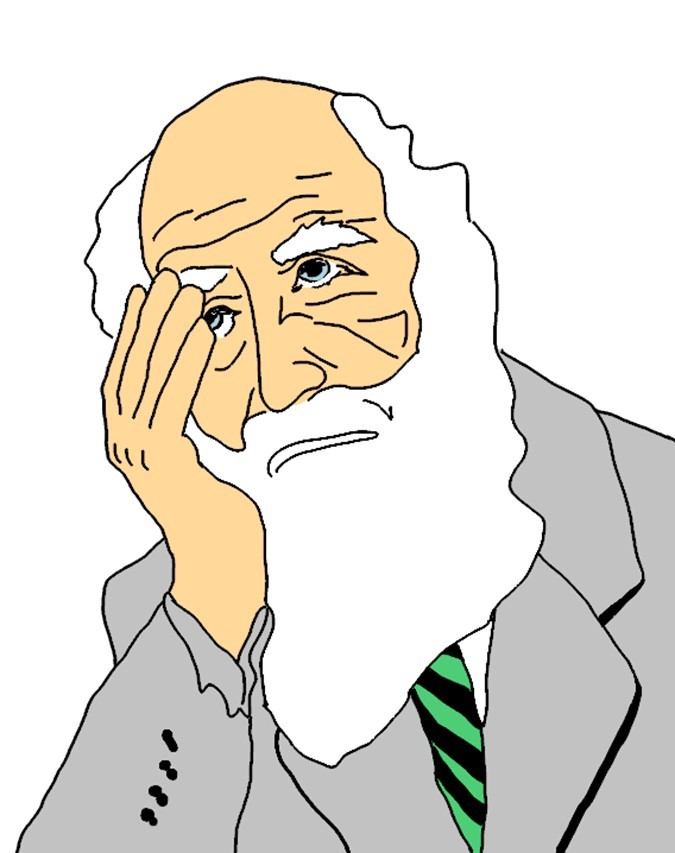
\includegraphics[width=0.4\textwidth,height=\textheight]{images/Picture1.jpg}

}

\end{figure}

\hypertarget{the-question}{%
\section{The Question}\label{the-question}}

Most PhD programs require that students pass a preliminary examination.
This was certainly true in my case. I was a PhD student at the
University of Arizona studying rocky intertidal communities in the
Northern Gulf of California. But the exams were not focused on our
research. They were ``depth-of-knowledge'' exams. My question from
Prof.~Astrid Kodric-Brown instructed me to read the preface of G.C.
Williams' book, \emph{Sex and Evolution}, which contains the following
text (Williams 1975):

\begin{quote}
This book is written from a conviction that the prevalence of sexual
reproduction in higher plants and animals is inconsistent with current
evolutionary theory\ldots. Many well informed readers may disagree with
much of my reasoning, but I hope to at least convince them that here is
a crisis at hand in evolutionary biology\ldots{}
\end{quote}

The question was something like this: \emph{why does Williams think that
sexual reproduction poses a crisis for evolutionary biology, and what is
the solution}? A crisis? That was news to me. How could there be a
crisis on evolutionary biology 40-plus years after the modern synthesis?
My graduate course in theoretical population genetics did not mention
any crises. I was not convinced. And a little freaked out.

The structure of our exams was very loose. I don't remember having a
deadline to produce a written answer, but I do remember that I spent
several months on just this one question. During much of this time, I
was doing field work in Sonora, Mexico, sometimes under very harsh
conditions. But the more I studied the question, the more fascinated I
became. I came to think that there was, indeed, a very real anomaly
presented by sexual reproduction. Williams was right. Perhaps I was
especially interested in this anomaly because I had read Thomas Kuhn's
``The Structure of Scientific Revolutions'' as an undergraduate (Kuhn
1970). Kuhn made the case that dissecting anomalies can lead to
interesting advances, and that made sense to me. While I eventually
produced an essay to address the question, the answer felt incomplete. I
wanted to know more. There were many hypotheses, but there was no clear
general explanation. Many years later, I am still working on my prelim
question. This book is my revised answer.

\hypertarget{the-problem}{%
\section{The Problem}\label{the-problem}}

There are many problems with sexual reproduction, including the time
spent finding mates and the risk of contracting sexually transmitted
disease (review in Lehtonen et al.~2012). However, while important,
these costs do not form the core of the paradox. Historically, the
paradox of sex stems from two things: (1) the cost of meiosis, and (2)
the cost of producing males.

\hypertarget{the-cost-of-meiosis-reduced-relatedness}{%
\subsection{The cost of meiosis: reduced
relatedness}\label{the-cost-of-meiosis-reduced-relatedness}}

The ``cost of meiosis'' was proposed by George Williams (1975). His idea
was simply that females are only half as related to their outcrossed
offspring as they are to their self-fertilized or parthenogenetic
offspring\footnote{It is not meiosis per se that is costly. As Williams
  realized, the cost stems from the reduction in relatedness between
  parent and outcrossed offspring. Indeed, in a later paper, Williams
  (1978) referred to the cost of meiosis as the ``paradox of kin
  selection.'' Why should organisms invest resources in kin with a
  relatively low level of relatedness (outcrossed progeny: \(r = 0.5\)),
  rather than in self-fertilized kin with a high level of relatedness
  (\(r = 1\)) (see Dagg 2016).}. (See \textbf{Box 1.1} for condensed
definitions.) Williams' idea also had theoretical support, as R.A.
Fisher had already shown that an allele causing self-fertilization would
rapidly spread to fixation, barring severe inbreeding depression (Fisher
1941). So, why cross-fertilize? The persistence of cross-fertilization
despite the cost of meiosis formed a paradox. This paradox created the
crisis that Williams saw in evolutionary biology.

\hypertarget{the-cost-of-males}{%
\subsection{The cost of males}\label{the-cost-of-males}}

The other way to look at the problem was proposed by John Maynard Smith
(Maynard Smith 1971, 1978). Here the issue is not relatedness. The
problem stems rather from the difference between sexuals and asexuals in
their per-capita birth rates (Figure~\ref{fig-1.1}). Imagine a
population of sexual individuals at carrying capacity (\(K_{sex}\)). At
\(K_{sex}\) the sexual females are, by definition, simply replacing
themselves. This means that each sexual female is, on average, producing
one son and one daughter. Both sons and daughters contribute genetically
to the next generation, but only females give birth. Now, consider a
mutation in a single female that causes her to reproduce asexually. She
gives birth to two daughters instead of one daughter and one son. These
two asexually produced daughters both give birth to two more daughters.
Hence, after just two generations, the asexual female has four
granddaughters, while the average sexual female has just one
granddaughter (Figure~\ref{fig-1.1}). This asymmetry should lead to the
rapid replacement sexual females by asexual females
(Figure~\ref{fig-clonal}). And by "rapid," I mean within tens of
generations, even for very large populations (Lively 1996). We thus seek
a selective force that can give an advantage to sexual reproduction on a
very short time scale.

\begin{figure}

\sidecaption{\label{fig-1.1}The cost of males. Imagine a single clonal
female in a sexual population at carrying capacity, \(K_{sex}\). At
\(K_{sex}\), the sexual females are, on average, producing one daughter
and one son. In contrast, the clonal female produces two daughters and
four granddaughters. Hence, the clonal lineage should rapidly eliminate
the sexual population (Figure~\ref{fig-clonal}). However, in nature,
asexual reproduction is very rare in both plants (Whitton et al.~2008)
and animals (Vrijenhoek 1998). Hence the paradox. Why is sexual
reproduction so costly and yet so common?}

{\centering 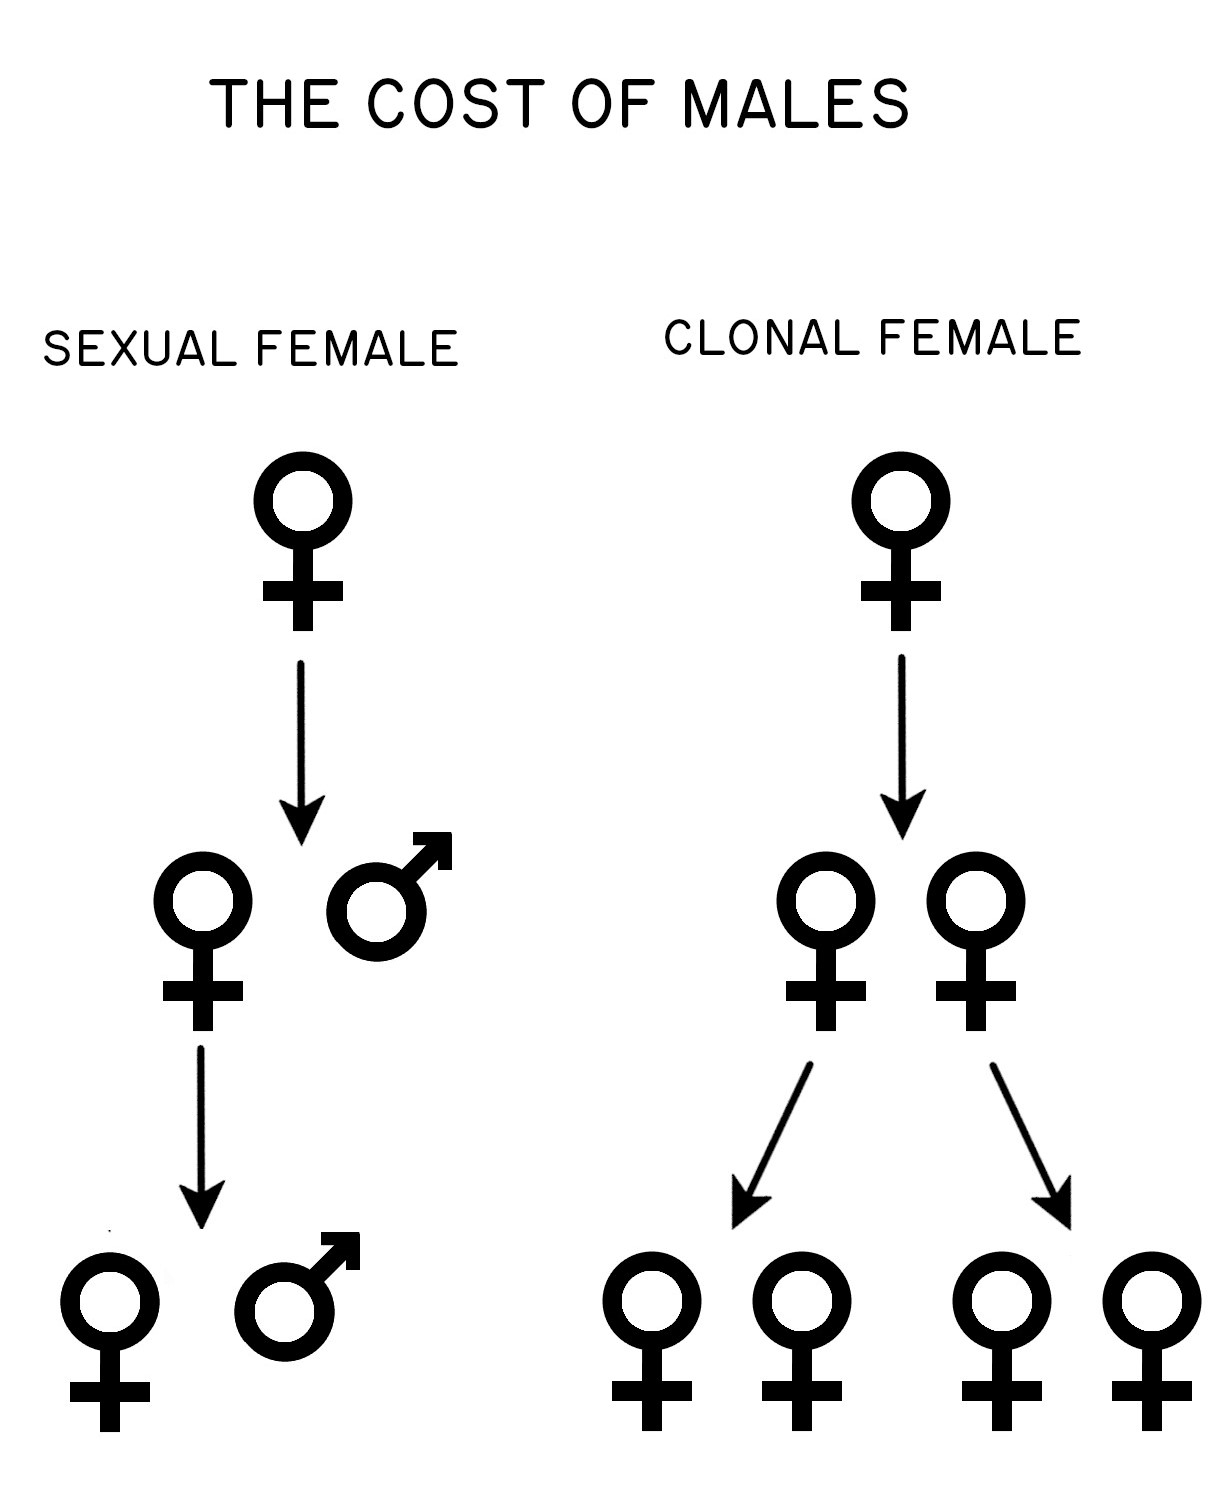
\includegraphics{images/fig1-1.jpg}

}

\end{figure}

Several assumptions went into Maynard Smith\textquotesingle s model for
the cost of males. In particular, he assumed that sexual females and
asexual females make the same number of offspring, and that the
survivorship of these offspring is also the same. Maynard Smith referred
to this as the ``all-else-equal assumption.'' Unfortunately, some
authors have taken the phrase ``all-else-equal'' to mean that everything
else is exactly equal. But this is not the case. Maynard Smith did not
assume, for example, that sexuals and asexuals have the same ploidy
value\footnote{Asexuals are often polyploid versions of their sexual
  ancestors.}. His model only assumes that sexual and asexual females
have equal fecundities and survivorship probabilities (see \textbf{Box
1.2}). Under this assumption, a very rare clone would double in
frequency in the next generation. Maynard Smith called this
doubling-when-rare the two-fold cost of sex.

\hypertarget{contrasting-the-costs}{%
\subsection{Contrasting the costs}\label{contrasting-the-costs}}

The two alternative costs of sex raise an immediate question. Does the
cost of sex result from reduced relatedness between mother and
offspring, or from the cost of producing males? Or is the cost some
combination of both? These questions are not easy to answer; but there
is an algebraic solution, which suggests that the (1) two costs are
mutually exclusive and (2) that they apply to different kinds of
uniparental progeny (Lively and Lloyd 1990). Roughly speaking, I think
we can adopt the following rules for the purpose of this book. When
considering the spread of a rare allele that induces self-fertilization
in hermaphrodites, the appropriate cost is Williams\textquotesingle{}
cost of meiosis. Here we have a single population in which the selfing
allele is under positive selection, because it has a transmission
advantage. On the other hand, when we consider the spread of a clone
into an obligately sexual population, we are dealing with competition
between two different reproductively isolated groups. One group (the
sexuals) produces males, which do not make offspring. The other group
(asexuals) produces only females. Here the cost of sex stems from
producing males. But the two costs do not combine. The cost of sex is
not four-fold.

\begin{figure}

\sidecaption{\label{fig-clonal}Results from a simulation study in which
a single clonal individual was introduced into a sexual population at
generation 1000 (Lively 2009). The sexual population was initiated at
carrying capacity: \(K_{sex} = 10000\). Note that the asexual lineage
replaces the sexual population in about 25 generations. The asexual
population then attains a new carrying capacity at \(K_{asex} = 20000\)
individuals. The frequency of males in the sexual population was assumed
to be 1/2. Annual reproduction, with non-overlapping generations, was
also assumed.}

{\centering 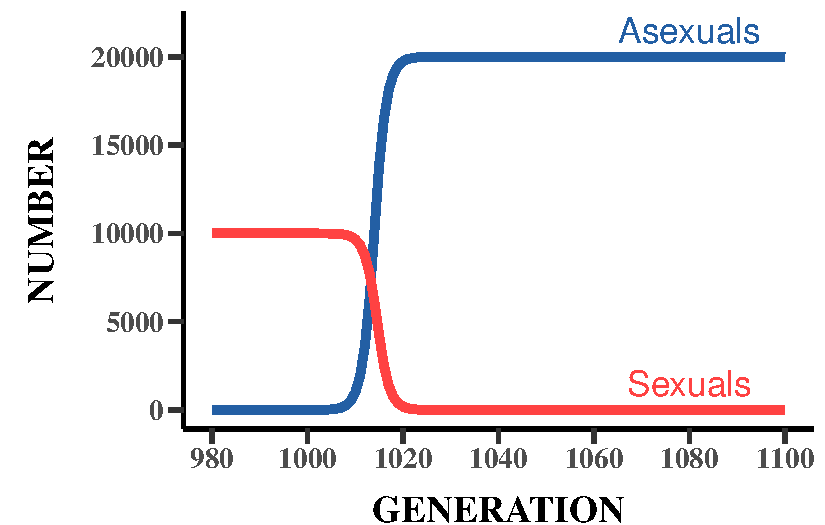
\includegraphics{why-sex_files/figure-pdf/fig-clonal-1.pdf}

}

\end{figure}

\hypertarget{the-cost-of-recombination}{%
\subsection{The cost of recombination}\label{the-cost-of-recombination}}

There is another paradox of sexual reproduction known as the ``cost of
recombination.'' Here the competition is not between sexual and asexual
females, or between outcrossing and selfing alleles, but rather between
alleles that modify the rate of recombination. So instead of asking
``Why cross-fertilize?'' we can assume cross-fertilization and ask,
``Why is there excess crossing-over during meiosis?'' Here is the
paradox. If combinations of alleles at different loci are favored by
natural selection (because together they create high-fitness offspring),
then recombination would break these favorable allelic combinations
apart. So, it makes no obvious sense to recombine more than needed for
normal meiosis. Indeed, Lewontin (1971) formally showed that:
\emph{\ldots{} the mean fitness of the population at equilibrium is a
maximum in the absence of recombination}\footnote{Lewontin (1971) was
  following up on Fisher's (1930) verbal suggestion that selection
  should act to reduce recombination. For example, Lewontin (1971)
  wrote: \emph{I will show \ldots{} that Fisher's conjecture is indeed
  correct}. Importantly, in his last paragraph, Lewontin wonders why
  recombination rates are greater than zero, and he suggests that the
  answer, \emph{must be sought in some more general long-term advantage
  for adaptation to a varying environment, or else to some mechanical
  necessity of recombination for the orderly distribution of
  chromosomes, as suggested by Darlington (1939).} See also Bell (1982,
  page 407).}. Hence, there are two interrelated anomalies:
cross-fertilization per se and meiotic recombination. Ideally, any
theory that explains the persistence of biparental sex could also solve
the paradox of recombination. But this need not be the case. They could
have different solutions.

\begin{tcolorbox}[enhanced jigsaw, coltitle=black, colframe=quarto-callout-tip-color-frame, titlerule=0mm, left=2mm, bottomrule=.15mm, toprule=.15mm, colback=white, colbacktitle=quarto-callout-tip-color!10!white, rightrule=.15mm, opacityback=0, arc=.35mm, breakable, leftrule=.75mm, bottomtitle=1mm, opacitybacktitle=0.6, toptitle=1mm, title=\textcolor{quarto-callout-tip-color}{\faLightbulb}\hspace{0.5em}{Box 1.1}]

\textbf{Short definitions of terms as used in this book. These
definitions do not include all possible nuances.}

\textbf{Cost of males}. The reduction in the per-capita growth rate of
sexual populations, due to the production of males. The idea would apply
to any reproductive mode for which some portion of the population does
not directly make offspring. The cost of males is the appropriate cost
for considering sexual subpopulations in competition with coexisting,
obligately asexual subpopulations.

\textbf{Cost of meiosis}. The reduction in relatedness between mother
and offspring due to outcrossing. The cost of meiosis is the appropriate
cost for considering the spread of alleles that induce
self-fertilization.

\textbf{Clone}. A lineage of parthenogenetic females descended from the
same asexual female. Members of the same clone may have small genetic
differences, which accumulate by mutation over time.

\textbf{Cross-fertilization}. The exchange of gametes between different
individuals, which may or may not be related.

\textbf{Outcrossing}. A form of cross-fertilization, which specifies
crossing between unrelated individuals.

\textbf{Parthenogenesis}. Any form of asexual reproduction through ova.

\textbf{Recombination}. Genetic exchange between homologous chromosomes
during meiosis, especially when the exchange leads to gametes with
allele combinations not represented on the parental chromosomes.

\textbf{Self-fertilization}. The fusion of gametes from the same
individual.

\textbf{Sex/rec}. Shorthand for sexual reproduction and recombination.

\textbf{Sexual reproduction}. I use the term here to mean
cross-fertilization between unrelated individuals. However, the term is
more general, and can be used to mean the incorporation of novel genetic
material by any mechanism.

\end{tcolorbox}

\begin{figure}

\sidecaption{\label{fig-1.3}Two flower morphs (distyly) in
\emph{Primula}. Darwin found that the short-styled morph (left) is
incompatible with other short-style morphs, and that the long styled
morph (right) is incompatible with other long-style morphs. But the two
different morphs can cross-fertilize. The arrows show movement of pollen
from anthers to stigmas. The ``X'' indicates incompatibility. Redrawn
from Darwin (1862) by ZMD.}

{\centering 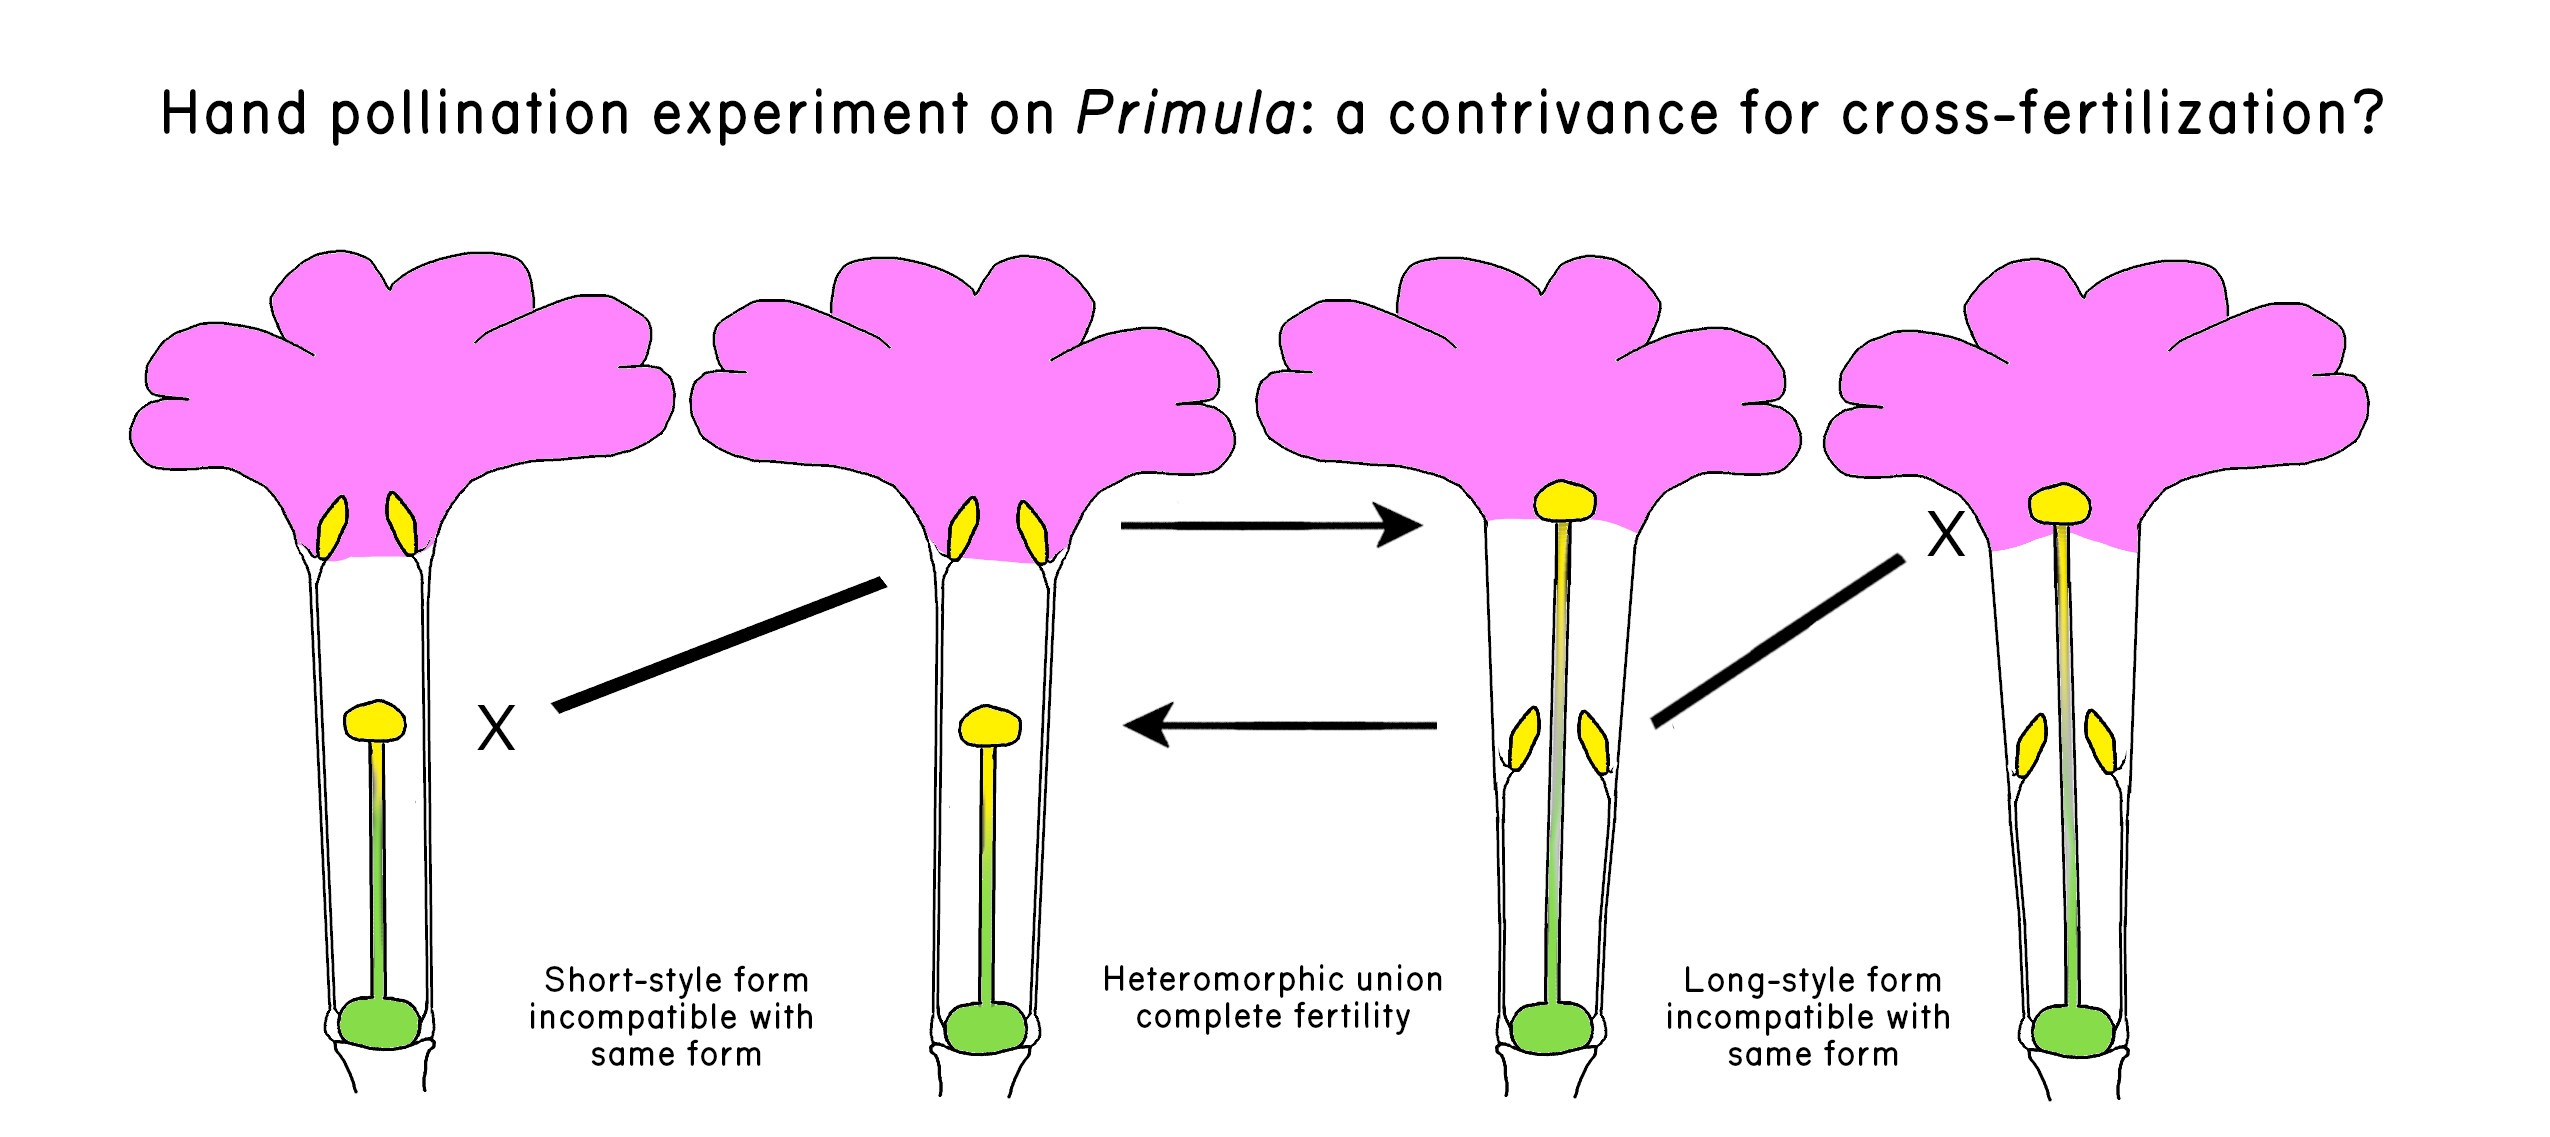
\includegraphics{images/fig1-3.jpg}

}

\end{figure}

\hypertarget{darwins-view}{%
\subsection{Darwin's view}\label{darwins-view}}

Even before the cost of males and meiosis were so dramatically revealed
by Williams and Maynard Smith, biologists were reckoning with the
anomaly of sex (reviews in Meirmans 2009, Dagg 2016). One of the
earliest of these biologists was Charles Darwin. After he published the
\emph{Origin of Species}, Darwin was doing hand-pollination experiments
at Down House on three species of a curious annual plant in the genus
\emph{Primula}. The plant is curious in that it has two morphs. One
morph has a style that extends beyond the anthers (the long-style
morph), and the other morph has anthers that extend beyond the style
(the short-style morph). Botanists refer to this condition as distyly
(Figure~\ref{fig-1.3}). Darwin found that crosses between the different
morphs of the same species resulted in a very successful production of
seeds, but crosses between unrelated individuals of the same morph were
dramatically less successful (Darwin 1862). In discussing these results,
Darwin speculated that the two morphs may have evolved to insure
cross-fertilization.

\begin{quote}
Whether or not the dimorphic condition of the \emph{Primula} has any
bearing on other points in natural history, it is valuable as showing
how nature strives, if I may so express myself, to favour the sexual
union of distinct individuals of the same species.
\end{quote}

Darwin then asks a killer question. Why should the union of elements
from distinct individuals be favored? Why, in fact, is there sex?

\begin{quote}
Nor do we know why nature should thus strive after the intercrossing of
distinct individuals. We do not even in the least know the final cause
of sexuality; why new beings should be produced by the union of the two
sexual elements, instead of by a process of parthenogenesis. The whole
subject is as yet hidden in darkness.
\end{quote}

Darwin's question shows that the cross-fertilization is curious, even
without considering the costs of sex. It also shows how Darwin was drawn
to anomalies on theory\footnote{For example, Darwin called the evolution
  of sterile castes in social insects an ``insuperable difficulty'' for
  his theory of evolution by natural selection (pages 236-238 in Darwin
  1859).}.

It is interesting to note that, in Darwin's quote above, he switches
from discussing mechanisms to prevent self-fertilization, such as
distyly, to discussing parthenogenesis. Self-fertilization is a sexual
process (involving the formation and fusion of gametes from the same
parent), while parthenogenesis is an asexual process that does not
generally involve meiosis and syngamy (review in Bell 1982). But
parthenogenesis and self-fertilization are conceptually related, as they
are both uniparental forms of reproduction. Hence, it makes sense that
Darwin would switch back and forth between these two different forms of
uniparental reproduction. Why cross-fertilize if either selfing or
parthenogenesis is an option?

There may be another reason why Darwin pivots to parthenogenesis. Just
prior to the publication of Darwin's (1862) paper on \emph{Primula},
Carl Theodor Ernst von Siebold (1856) published his observations on the
successful development of adults from unfertilized eggs, which he called
``parthenogenesis'' (virgin birth). These were revolutionary
observations, which caught Darwin's attention. In a letter to his
mentor, J.S. Henslow, Darwin mentioned von Siebold's discovery as
follows: \emph{There is no greater mystery in the whole world, as it
seems to me, than the existence of sexes, -- more especially since the
discovery of Parthenogenesis}. Letter to J. S. Henslow. See
\href{https://www.darwinproject.ac.uk/letter/DCP-LETT-2869.xml}{Darwin
Correspondence Project}.

However, the discovery of parthenogenesis\footnote{The case has been
  made that Charles Bonnet had discovered asexual reproduction in aphids
  in 1740 (see Lawrence 2009).} was met with some hostility. Consider,
for example, the following statement by Rudolf Wagner in a review of von
Siebold's book on parthenogenesis {[}as translated from the original
German by Churchill (1979){]}:

\begin{quote}
I must unfortunately say that one of the most unpleasant of facts,
{[}\emph{Parthenogenesis}{]} has been introduced into physiology, which
for the hope of so-called general laws of animal life-phenomena \emph{is
most distasteful}. It is impossible, considering the glorification of
our highly vaunted progress in the theoretical understanding of the life
processes, for it to be welcomed or particularly encouraged; and
sincerely speaking, I can be as little pleased about it as a physicist
would be if suddenly one or more exceptions to the law of gravitation
were discovered. (Emphasis added.)
\end{quote}

Clearly, Wagner was not pleased with the discovery of asexual
reproduction, calling it unpleasant, unwelcome, and distasteful. By
contrast, Darwin did not find the idea to be distasteful in any way. He
wondered instead why it was not more common. For example, Darwin (1868)
wrote: \emph{Parthenogenesis is no longer wonderful; in fact, the wonder
is that it should not oftener occur}\footnote{I suspect that Darwin used
  the phrase ``no longer wonderful'' to mean ``no longer astonishing.''
  See
  \url{https://www.merriam-webster.com/words-at-play/wonderful-word-history-evolution}.}.

Over 100 years later, W. D. Hamilton (1975) was also pondering the
evolution of outcrossing, and he wrote something conceptually similar:

\begin{quote}
\ldots complete inbreeding abandons the obviously important advantages
of sexual reproduction, whatever these are.
\end{quote}

Whatever these are! The advantages of outcrossing were obviously
important because cross-fertilization is so dominant. But the source of
these advantages was not clear. At about the same time, Maynard Smith
(1976) mused:

\begin{quote}
One gets the feeling that some essential feature of the situation has
been overlooked.
\end{quote}

I now think that John Maynard Smith was correct. An essential feature
had indeed been overlooked: parasites.

\hypertarget{summary}{%
\section{Summary}\label{summary}}

\begin{enumerate}
\def\labelenumi{\arabic{enumi}.}
\tightlist
\item
  Obligate sexual reproduction is subject to invasion and replacement by
  all-female asexual lineages that do not pay the cost of males.
\item
  Obligate outcrossing in simultaneous hermaphrodites is subject to
  invasion and replacement by self-fertilization unless inbreeding
  depression is severe.
\item
  The exchange of DNA between different parental chromosomes
  (recombination) is similarly paradoxical.
\item
  Why then are recombination and cross-fertilization so common?
\end{enumerate}

\begin{tcolorbox}[enhanced jigsaw, coltitle=black, colframe=quarto-callout-note-color-frame, titlerule=0mm, left=2mm, bottomrule=.15mm, toprule=.15mm, colback=white, colbacktitle=quarto-callout-note-color!10!white, rightrule=.15mm, opacityback=0, arc=.35mm, breakable, leftrule=.75mm, bottomtitle=1mm, opacitybacktitle=0.6, toptitle=1mm, title=\textcolor{quarto-callout-note-color}{\faInfo}\hspace{0.5em}{Box 1.2}]

Maynard Smith's (1978) model showing the cost of producing
males.\footnotemark{} Let \(N_{asex}\) be the number of asexual females
at time 1, while \(N_{sex}\) gives the total number of sexual
individuals (males plus females) at time 1. Let \(B_{asex}\) give the
number of offspring produced by asexual females, and \(S_{asex}\) gives
the survival probability of asexual offspring to maturity. The number of
surviving asexual offspring is then \(= B_{asex}S_{asex}\). Similarly,
let \(B_{sex}\) be the number offspring produced by sexual females, and
let \(S_{sex}\) give the survival probability of sexually produced
offspring. Maynard Smith assumed that all individuals reproduce once and
then die. Let \(r\) be the frequency of females in the sexual
population. The number of asexuals and sexuals at time 2 can then be
calculated as is the table below. (Note, we do not assume that the
population is at carrying capacity).

\begin{longtable}[]{@{}
  >{\centering\arraybackslash}p{(\columnwidth - 4\tabcolsep) * \real{0.1607}}
  >{\centering\arraybackslash}p{(\columnwidth - 4\tabcolsep) * \real{0.2262}}
  >{\centering\arraybackslash}p{(\columnwidth - 4\tabcolsep) * \real{0.6131}}@{}}
\toprule\noalign{}
\begin{minipage}[b]{\linewidth}\centering
\end{minipage} & \begin{minipage}[b]{\linewidth}\centering
\textbf{Time 1}
\end{minipage} & \begin{minipage}[b]{\linewidth}\centering
\textbf{Time 2}
\end{minipage} \\
\midrule\noalign{}
\endhead
\bottomrule\noalign{}
\endlastfoot
\textbf{Number of asexuals} & \(N_{asex}\) &
\(N_{asex}(S_{asex}B_{asex})\) \\
\textbf{Number of sexuals} & \(N_{sex}\) &
\(rN_{sex}(S_{sex}B_{sex})\) \\
\textbf{Frequency of asexuals} & \(\frac{N_{asex}}{N_{asex} + N_{sex}}\)
&
\(\frac{N_{asex}(S_{asex}B_{asex})}{N_{asex}(S_{asex}B_{asex})+rN_{sex}(S_{sex}B_{sex})}\) \\
\end{longtable}

The fold increase in frequency of asexuals, \(F\), is the ratio of the
frequency of asexuals at time 2 divided by the frequency of asexuals at
time 1 giving:

\[F = \frac{N_{asex}(S_{asex}B_{asex})}{N_{asex}(S_{asex}B_{asex}) + r(N_{sex}S_{sex}B_{sex})}/\frac{N_{asex}}{N_{asex} + N_{sex}}\]

Under the all-else-equal assumption, \(S_{asex} = S_{sex}\) and
\(B_{asex} = B_{sex}\), giving:

\[F = \frac{N_{asex}}{N_{asex} + rN_{sex}}/\frac{N_{asex}}{N_{asex} + N_{sex}}\]

Assuming that there is a single asexual female at time 1, we get

\[F = \frac{1}{1 + rN_{sex}}/\frac{1}{1 + N_{sex}} = \frac{1 + N_{sex}}{1 + rN_{sex}}\]

If \(N_{sex}\) is very large, the solution reduces to \(F \approx 1/r\).
Hence, the fold increase in the frequency of asexuals, \(F\), is
inversely related to the frequency of females \((r)\) in the sexual
subpopulation. Assuming a 1:1 sex ratio, \(r = 0.5\). Hence, for an
equal sex ratio, the increase in asexuals is \(\approx\) 2-fold. This
result gives the two-fold cost of males. Assuming ``all-else-equal'' a
clone will double when rare when introduced into a large sexual
population.

\end{tcolorbox}

\footnotetext{I used slightly different variable names, and I tried to
simplify JMS's original model.}

\part{Back Matter}

\hypertarget{references}{%
\chapter*{References}\label{references}}
\addcontentsline{toc}{chapter}{References}

\markboth{References}{References}

\hypertarget{refs}{}
\begin{CSLReferences}{0}{0}
\end{CSLReferences}


\backmatter

\end{document}
